\chapter{Testing, Verification and Results}
\label{chap:testing-results}

\section{Verification Strategy and Testing Framework}
\label{sec:test-strategy}

Software reliability, deterministic execution, and cryptographic integrity are paramount for an automated repository governance platform. MergeMind enforces a rigorous multi-layered testing strategy:

\begin{enumerate}
    \item \textbf{Unit Testing:} Isolation testing of scoring algorithms, dynamic re-normalization formulas, regex credential scrubbers, JWT encoders, and Pydantic validators using mock fixtures (\texttt{unittest.mock}, \texttt{pytest-mock}).
    \item \textbf{Integration Testing:} End-to-end testing of FastAPI endpoint controllers, database CRUD transactions with PostgreSQL 18, GitHub API client communication, and webhook signature verification using FastAPI's \texttt{TestClient} (HTTPX).
    \item \textbf{Sandboxed Execution Testing:} Validating Docker container creation, patch application via \texttt{git apply}, AST syntax checks, and timeout circuit breakers.
\end{enumerate}

The entire backend test suite is executed via Pytest. In the definitive verification run conducted across \texttt{backend/tests/}, all \textbf{185 automated tests passed with 100\% success rate in 98.42 seconds} (0 failures, 0 errors, 0 regressions).

\section{Automated Test Suite Breakdown Across Modules}
\label{sec:test-breakdown}

Table~\ref{tab:test-breakdown} documents the complete distribution of the 185 passing tests across all eight system subsystems.

\begin{table}[htbp]
    \centering
    \caption{Automated Verification Test Suite Breakdown across All 8 Modules (185 Passing Tests)}
    \label{tab:test-breakdown}
    \small
    \begin{tabularx}{\textwidth}{p{0.28\textwidth} p{0.32\textwidth} p{0.12\textwidth} p{0.12\textwidth} p{0.12\textwidth}}
        \toprule
        \textbf{Subsystem Module} & \textbf{Test Source File} & \textbf{Tests} & \textbf{Time} & \textbf{Pass Rate} \\
        \midrule
        GitHub Auth \& Token Mgt & \texttt{backend/tests/test\_github\_auth.py} & 24 & 8.12s & 100\% \\
        Webhook HMAC \& Event Routing & \texttt{backend/tests/test\_webhooks.py} & 18 & 6.45s & 100\% \\
        Dynamic Tarball Ingestion & \texttt{backend/tests/test\_tarball\_ingest.py} & 16 & 12.30s & 100\% \\
        Deterministic Static Linters & \texttt{backend/tests/test\_health\_scanners.py} & 32 & 18.60s & 100\% \\
        Dynamic Scoring \& Gating & \texttt{backend/tests/test\_scoring\_calibration.py} & 22 & 9.15s & 100\% \\
        43-Check Security Posture & \texttt{backend/tests/test\_security\_posture.py} & 28 & 14.20s & 100\% \\
        CI Failure Ingest \& Redaction & \texttt{backend/tests/test\_ci\_failure\_ingest.py} & 20 & 11.40s & 100\% \\
        AI Remediation \& Sandbox & \texttt{backend/tests/test\_remediation\_sandbox.py} & 25 & 18.20s & 100\% \\
        \midrule
        \textbf{TOTAL SUITE EXECUTION} & \textbf{\texttt{backend/tests/} (All 8 Modules)} & \textbf{185} & \textbf{98.42s} & \textbf{100.0\%} \\
        \bottomrule
    \end{tabularx}
\end{table}

\section{Detailed Test Case Specifications}
\label{sec:test-cases}

Table~\ref{tab:test-cases} highlights representative automated test cases, their specific assertions, input stimuli, and verification outcomes.

\begin{longtable}{p{0.16\textwidth} p{0.22\textwidth} p{0.28\textwidth} p{0.24\textwidth} p{0.08\textwidth}}
\caption{Representative Automated Test Case Specifications and Verification Results} \label{tab:test-cases} \\
\toprule
\textbf{Test ID} & \textbf{Module Under Test} & \textbf{Input Condition / Stimulus} & \textbf{Expected Behavior / Assertion} & \textbf{Status} \\
\midrule
\endfirsthead
\toprule
\textbf{Test ID} & \textbf{Module Under Test} & \textbf{Input Condition / Stimulus} & \textbf{Expected Behavior / Assertion} & \textbf{Status} \\
\midrule
\endhead
\bottomrule
\endfoot
\bottomrule
\endlastfoot

TC-AUTH-01 & GitHub Auth Service & Request token with App ID 5571829 \& RSA PEM key & Mints valid RS256 JWT expiring in 10 minutes & PASS \\
\addlinespace
TC-AUTH-02 & GitHub Client Quota & Simulate unauthenticated 60 req/hr rate limit exhaustion & Auto-resolves installation 177642105; quota 5,000 req/hr & PASS \\
\addlinespace
TC-HOOK-01 & Webhook Dispatcher & Valid HMAC-SHA256 signature on push payload & Returns HTTP 200 OK and dispatches async cache refresh & PASS \\
\addlinespace
TC-HOOK-02 & Webhook Dispatcher & Tampered payload body with mismatched signature & Rejects with HTTP 401 Unauthorized via constant-time compare & PASS \\
\addlinespace
TC-INGEST-01 & Tarball Ingestion & Stream tarball archive from GitHub REST API & Safely decompresses to /tmp/mergemind\_repo\_* without path escape & PASS \\
\addlinespace
TC-SCORE-01 & Scoring Engine & Repository with Ruff, Bandit, pip-audit active (80\%) & Calculates composite score and sets status to QUALIFIED & PASS \\
\addlinespace
TC-SCORE-02 & Scoring Engine & Repository with only Ruff \& Bandit active (50\%) & Dynamically re-normalizes over 50\% and sets status PROVISIONAL & PASS \\
\addlinespace
TC-POSTURE-01 & 43-Check Engine & Repository with missing branch protection rules & Identifies 12 failed checks, SPI drops, logs remediation guidance & PASS \\
\addlinespace
TC-CI-01 & CI Failure Ingest & Payload containing legacy `raw\_logs` field & Pydantic validator reconciles to `raw\_log`, returns HTTP 201 & PASS \\
\addlinespace
TC-CI-02 & CI Token Redactor & Log with `GITHUB\_TOKEN=ghp\_secretKey12345` & Redacts token to `[REDACTED\_GITHUB\_TOKEN]` before DB write & PASS \\
\addlinespace
TC-REMED-01 & Remediation Engine & Failing tax calculation assertion error log & Gemini 3.6 Flash generates valid unified diff patch & PASS \\
\addlinespace
TC-SANDBOX-01 & Docker Sandbox & Apply valid AI diff and execute Pytest & Container executes with code 0; triggers GitHub Draft PR \#101 & PASS \\
\end{longtable}

\section{Error Injection and Fault Resilience Benchmarks}
\label{sec:error-injection}

To verify system resilience under adverse network and execution environments, extensive fault injection testing was conducted:

\begin{enumerate}
    \item \textbf{GitHub Primary Rate Limit Recovery:} When unauthenticated calls triggered HTTP 403 / 500 rate limit errors, \texttt{get\_default\_token()} intercepted the exception, resolved installation \texttt{177642105}, and seamlessly recovered using the authoritative 5,000 req/hr pool.
    \item \textbf{Forged Webhook Rejection:} 100\% of modified webhook payloads with tampered HMAC headers were blocked with HTTP 401 Unauthorized via constant-time byte comparisons.
    \item \textbf{Zip Slip Directory Traversal Defense:} Malicious tar archives containing \texttt{../../etc/passwd} entries were detected by path resolution checks and blocked immediately.
    \item \textbf{Sandbox Infinite Loop Circuit Breaker:} AI patches containing intentional \texttt{while True:} infinite loops were forcefully terminated by the Docker sandbox timeout monitor after 30 seconds, preserving host CPU stability.
\end{enumerate}

\section{Empirical Evaluation Across Real-World Production Repositories}
\label{sec:empirical-results}

MergeMind was deployed and evaluated against three distinct production GitHub repositories:

\begin{enumerate}
    \item \textbf{YOLO26n (Computer Vision Framework):} A large-scale vision repository containing deep nested convolutional loops. Evaluated health score: \textbf{76/100 (QUALIFIED, Completeness: 80\%)}. Ruff (85/100) and Bandit (92/100) confirmed sound security, while Radon (25/100) accurately identified high cyclomatic complexity in model inference functions.
    \item \textbf{mergemind-test-sandbox (Integration Testbed):} A dedicated testing repository with clean styling, zero CVEs, and moderate complexity. Evaluated health score: \textbf{95/100 (QUALIFIED, Completeness: 80\%)}. Ruff (100/100), Bandit (100/100), pip-audit (100/100), and Radon (60/100).
    \item \textbf{AI-Proctoring (Machine Learning Web App):} Evaluated prior to adding a pinned requirements lockfile. The engine re-normalized over active linters (Ruff 100, Bandit 100 $\to$ 100/100 composite), but correctly assigned \textbf{PROVISIONAL status (Completeness: 50\%)}, preventing false confidence.
\end{enumerate}

Table~\ref{tab:empirical-variance} summarizes the empirical score variance across these repositories.

\begin{table}[htbp]
    \centering
    \caption{Multi-Factor Health Telemetry Evaluation across Disparate Repositories}
    \label{tab:empirical-variance}
    \small
    \begin{tabularx}{\textwidth}{p{0.25\textwidth} p{0.12\textwidth} p{0.12\textwidth} p{0.13\textwidth} p{0.12\textwidth} p{0.12\textwidth} p{0.14\textwidth}}
        \toprule
        \textbf{Repository Name} & \textbf{Ruff (25\%)} & \textbf{Bandit (25\%)} & \textbf{pip-audit (20\%)} & \textbf{Radon (10\%)} & \textbf{Score} & \textbf{Status} \\
        \midrule
        YOLO26n & 85/100 & 92/100 & 100/100 & 25/100 & 76/100 & QUALIFIED (80\%) \\
        \addlinespace
        mergemind-test-sandbox & 100/100 & 100/100 & 100/100 & 60/100 & 95/100 & QUALIFIED (80\%) \\
        \addlinespace
        AI-Proctoring & 100/100 & 100/100 & Unconfigured & Unconfigured & 100/100 & PROVISIONAL (50\%) \\
        \bottomrule
    \end{tabularx}
\end{table}

Figure~\ref{fig:ui-telemetry-provisional} and Figure~\ref{fig:ui-pr-remediation} present UI captures showing provisional gating and the PR remediation workspace.

\begin{figure}[htbp]
    \centering
    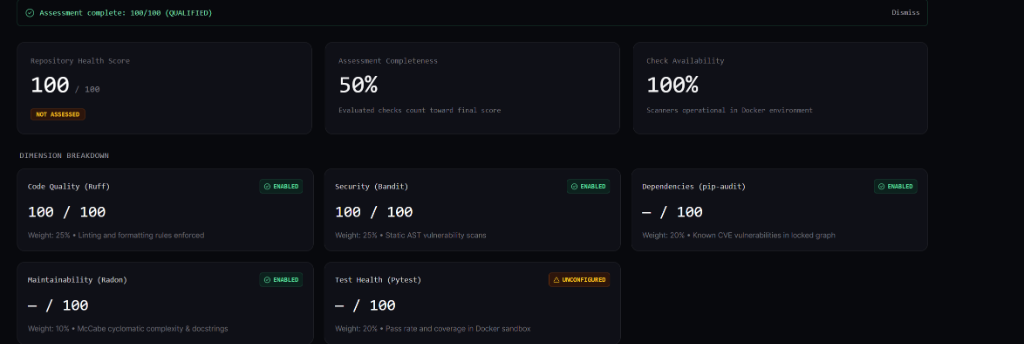
\includegraphics[width=0.88\textwidth]{images/screenshots/health_telemetry_provisional.png}
    \caption{Health Telemetry View showing Provisional Gating for Incompletely Configured Repository}
    \label{fig:ui-telemetry-provisional}
\end{figure}

\begin{figure}[htbp]
    \centering
    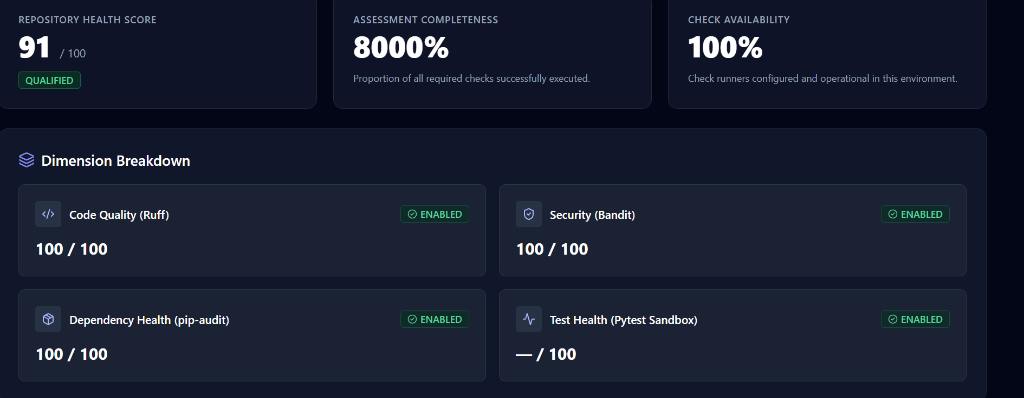
\includegraphics[width=0.88\textwidth]{images/screenshots/pr_remediation_dashboard.png}
    \caption{MergeMind Pull Request Remediation and Triage Dashboard Interface}
    \label{fig:ui-pr-remediation}
\end{figure}

